\documentclass[11pt,a4paper,titlepage]{article}

\usepackage[utf8]{inputenc}
\usepackage[T1]{fontenc}
\usepackage[slovene]{babel}
\usepackage{amsmath}
\usepackage{amssymb}
\usepackage[margin=3cm]{geometry}
\usepackage{graphicx}
\usepackage{float}
\usepackage[backend=biber, style=numeric]{biblatex}
\addbibresource{viri.bib}


\newcommand{\program}{Finančna matematika} % ime studijskega programa: Matematika/Finančna matematika
\newcommand{\imeavtorja}{Benjamin Levičar, Jan Nabergoj} % ime avtorja
\newcommand{\imementorja}{doc. dr. Janoš Vidali} % akademski naziv in ime mentorja
\newcommand{\imesomentorja}{prof. dr. Riste Škrekovski}
\newcommand{\naslovdela}{Pakirno kromatično število subdivizij subkubičnih grafov}
\newcommand{\letnica}{2025} %letnica 

\begin{document}
	
	%naslovnica
	
	\thispagestyle{empty}
	\noindent{\large
		UNIVERZA V LJUBLJANI\\[1mm]
		FAKULTETA ZA MATEMATIKO IN FIZIKO\\[5mm]
		\program\ }
	\vfill
	
	\begin{center}{\large
			\imeavtorja\\[2mm]
			{\bf \naslovdela}\\[10mm]
			Mentorja: \imementorja, \\ \imesomentorja\\[2mm]}
	\end{center}
	\vfill
	
	\noindent{\large
		Ljubljana, januar \letnica}
	\pagebreak



\section{Osnovne definicije in opis problema}

\subsection{Definicije}

\begin{itemize}
    \item \emph{Subkubičen graf} je graf v katerem imajo vsa vozlišča stopnjo največ 3.
    \item Imejmo graf $G=(V, E)$. \emph{Subdivizijo povezave} $uv\in E$ dobimo tako, da jo odstranimo in dodamo novo vozlišče $w$ ter povezavi
          $uw$, $wv$. \emph{Subdivizija grafa} $G$ je graf, ki ga dobimo da subdividiramo nekatere njegove povezave. Za naše namene bomo z $S(G)$
          označili graf, ki ga dobimo, če v $G$ subdividiramo vse povezave natanko enkrat.
    \item Naj bo $G=(V, E)$ graf in $i\in \mathbb{N}$, \emph{i-pakirnaje} grafa $G$ je množica $X \subseteq V$, tako da za poljubni 
          vozlišči $u, v\in X$ velja $d_G(u, v) > i$. \emph{Pakirno kromatično število} grafa $G$ je najmanjše število $k$, tako da se lahko dobi
          particijo $X_1, X_2, \dots, X_k$ množice $V$ in da je $X_i$ $i$-pakiranje za vsak $i\in \{1, 2, \dots, k\}$. Označimo ga z $\chi_\rho(G)$.

\end{itemize}
\begin{figure}[h]
	\centering
	\begin{minipage}{0.45\textwidth}
		\centering
		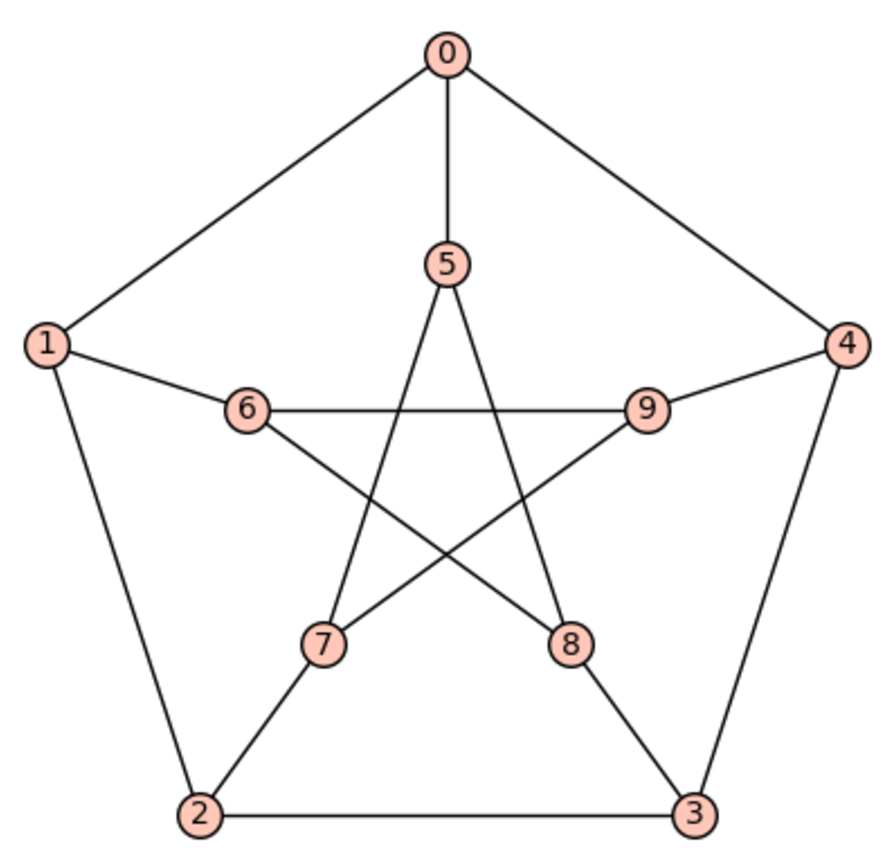
\includegraphics[width=\linewidth]{petersen_graph.png}
		\caption{Petersenov graf}
	\end{minipage}
	\hfill
	\begin{minipage}{0.45\textwidth}
		\centering
		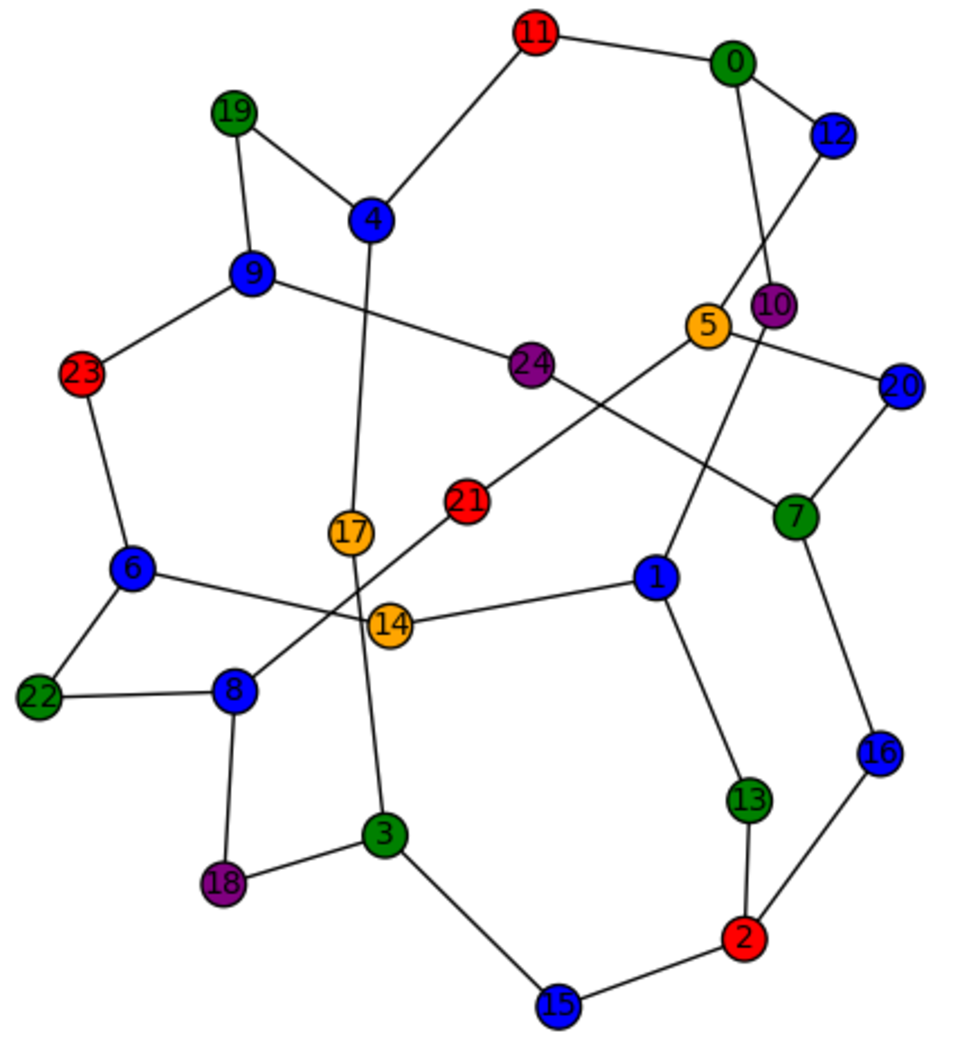
\includegraphics[width=\linewidth]{subdivizija_petersen_graph.png}
		\caption{Barvanje subdivizije petersenovega grafa}
	\end{minipage}
\end{figure}


\subsection{Opis problema}

Preveriti  želimo domnevo: \emph{Za vsako subdivizijo subkubičnega grafa $G$ velja $\chi_\rho(S(G)) \leq 5$}. Tega se bomo lotili z iskanjem protiprimera, torej želimo poiskati subdivizijo subkubičnega grafa, ki ima pakirno kromatično število vsaj 6. Na manjših grafih se problema lotimo sistematično in preverimo vse povezane subkubične grafe. Ker število grafov narašča eksponentno z številom vozlišč, pri večjem številu vozlišč pa iščemo s pomočjo stohastičnega iskanja.


\section{Sistematično iskanje}

\subsection{CLP}

Za izračun pakirnega kromatičnega števila sva implementirala sledeči celoštevilski linearni program iz \cite{SHAO20153588}: \\
imejmo graf $G=(V, E)$ za vozlišče $v \in V$ in $i \in \{1, 2, \dots, k\}$ naj bo $x_{v, i}$ enak $1$, če je $v$ pobarvano z barvo $i$ in 
$0$ sicer, $k$ je največje število dovoljenih barv. Naj bo $z$ največje število uporabljenih barv. 

\begin{align}
      \label{eq:f.0} \mbox{min}~& \;z& \\
      \label{eq:f.1} \mbox{p.p. } &\sum_{i=1}^{k} x_{v, i} = 1  & \forall v\in V(G)\\
      \label{eq:f.2}&x_{v, i} + x_{u, i} \leq 1& d_G(u, v) \leq i, \forall u, v\in V(G), 1 \leq i \leq k\\
      \label{eq:f.3}&i x_{v, i} \leq z & \forall v \in V(G), 1 \leq i \leq k\\
      \label{eq:f.4}&x_{v, i} \in \{0, 1\} & \forall v \in V(G), 1 \leq i \leq k
\end{align}
Pogoj $(2)$ poskrbi, da je vsako vozlišče pobarvano z natanko eno barvo. \\
Pogoj $(3)$ poskrbi, da sta vozlišči pobarvani z različnima barvama, če je $d_G(u, v) \leq i$. \\
Pogoj $(4)$ poskrbi, da je vsako vozlišče pobarvano z barvo $\leq z$.\\
Pogoj $(5)$ določi dovoljene vrednosti za spremenljivke $x_{v, i}$.

\subsection{Generiranje grafov}
Za generiranje subkubičnih grafov sva uporabila funkcijo \emph{nauty\_geng} z omejitvami, da mora biti graf povezan ter najvišja stopnja vozlišča je 3. Pakirno kromatično števlilo dobljenih grafov sva dobila z uporabo že zgoraj navedenega CLP. S tem sva preverila vse grafe na do vkjučno 14 vozlišč. Grafa katerega subdivizija bi imela pakirno kromatično število 6 ali več na tako malo vozliščih nisva našla.

\subsection{Lastnosti grafov z pakirnim kromatičnim števiom 5}
Odločila sva se, da pregledava lastnosti grafov katerih subdivizije imajo do sedaj največjo najdeno pakirno kromatično število 5 in si znjimi pomagava pri nadaljnem iskanju. Preverjala sva dvodelnost, ravninskost, gostoto, zgoščenost, premer, \dots.\\
Definicije lastnosti:
\begin{itemize}
	\item \emph{Dvodelnost:} Graf je dvodelen, če lahko njegova vozlišča razdelimo v dve skupini tako, da vozlišča v isti skupini med seboj niso povezana. To pomeni, da ga lahko z klasičnim barvanjem pobarvamo z dvema barvama.
	\item  \emph{Ravninskost:} Graf je ravninski, če lahko narišemo vse njegove povezave brez, da bi se sekale. Primer neravninskega grafa je $K_{3,3}$.
	\item  \emph{Zgoščenost:} meri, kako verjetno so sosednja vozlišča povezana med seboj. Izračunamo pa formuli $C_v = \frac{2E_v}{k_v(k_v-1)}$ za vozlišče $v$. Z $E_v$ število povezav med sosedi in $\frac{k_v(k_v-1)}{2}$ pa število vseh možnih povezav na grafu. To naredimo za vsako vozlišče in povprečimo.
	\item \emph{Povprečna razdalja:} nam pove koliko so v povprečju vozlišča v grafu narazen. To poračunamo preko matkike razdalj.
	\item  \emph{Premer:} je najdaljša najkrajša razdalja med dvema vozliščema v grafu. 
\end{itemize}



\subsubsection{8 vozlišč}
Od 196 najdenih grafov je 6 grafov katerih subdivizije imajo pakirno kromatično število 5. Kar je 3\%. 
\begin{table}[H]
	\begin{tabular}{|l|l|l|l|l|l|}
		\hline
		Število dvodelnih	& Število ravninskih  & Gostota  & Zgoščenost & Povprečna razdalja & Premer \\ \hline
		0 & 4 & 1.0 & 0.09 & 1.95 & 3.67  \\ \hline
	\end{tabular}
\end{table}

\subsubsection{9 vozlišč}
Od 531 najdenih grafov je 13 grafov katerih subdivizije imajo pakirno kromatično število 5. Kar je 2,4\%.  
\begin{table}[H]
	\begin{tabular}{|l|l|l|l|l|l|}
		\hline
		Število dvodelnih	& Število ravninskih  & Gostota  & Zgoščenost & Povprečna razdalja & Premer \\ \hline
		0 & 11  & 0.89 & 0.13 & 2.12 & 4.07 \\ \hline
	\end{tabular}
\end{table}

\subsubsection{10 vozlišč}
Od 1733 najdenih grafov je 42 grafov katerih subdivizije imajo pakirno kromatično število 5. Kar je 2,4\%.
\begin{table}[H]
	\begin{tabular}{|l|l|l|l|l|l|}
		\hline
		Število dvodelnih	& Število ravninskih  & Gostota  & Zgoščenost & Povprečna razdalja & Premer \\ \hline
		0 & 34  & 0.98 & 0.11 & 2.3 & 4.8 \\ \hline
	\end{tabular}
\end{table}

\subsubsection{11 vozlišč}
Od 5524 najdenih grafov je 99 grafov katerih subdivizije imajo pakirno kromatično število 5. Kar je 1,7\%. 
\begin{table}[H]
	\begin{tabular}{|l|l|l|l|l|l|}
		\hline
		Število dvodelnih	& Število ravninskih  & Gostota  & Zgoščenost & Povprečna razdalja & Premer \\ \hline
		0 & 80  & 0.88 & 0.12 & 2.5 & 5.27 \\ \hline
	\end{tabular}
\end{table}

\subsubsection{12 vozlišč}
Od 19430 najdenih grafov je 365 grafov katerih subdivizije imajo pakirno kromatično število 5. Kar je 1,8\%. 
\begin{table}[H]
	\begin{tabular}{|l|l|l|l|l|l|}
		\hline
		Število dvodelnih	& Število ravninskih  & Gostota  & Zgoščenost & Povprečna razdalja & Premer \\ \hline
		0 & 294  & 0.95 & 0.12 & 2.64 & 5.64 \\ \hline
	\end{tabular}
\end{table}

\subsubsection{13 vozlišč}
Od 69322 najdenih grafov je 1021 grafov katerih subdivizije imajo pakirno kromatično število 5. Kar je 1,4\%.

\begin{table}[H]
	\begin{tabular}{|l|l|l|l|l|l|}
		\hline
		Število dvodelnih	& Število ravninskih  & Gostota  & Zgoščenost & Povprečna razdalja & Premer \\ \hline
		0 & 819 & 0.87 & 0.11 & 2.83 & 6.18 \\ \hline
	\end{tabular}
\end{table}
\subsubsection{14 vozlišč}
Od 262044 najdenih grafov je 3680 grafov katerih subdivizije imajo pakirno kromatično število 5. Kar je 1,4\%
\begin{table}[H]
	\begin{tabular}{|l|l|l|l|l|l|}
		\hline
		Število dvodelnih	& Število ravninskih  & Gostota  & Zgoščenost & Povprečna razdalja & Premer \\ \hline
		0 & 2813 & 0.94 & 0.11 & 2.96 & 6.47 \\ \hline
	\end{tabular}
\end{table}

\subsection{Ugotovitve sistematičnega iskanja}
Opazimo lahko, da noben graf kateraga subdivizija ima pakirno kromatično barvanje enako 5 ni dvodelen. Če pomislimo zakaj, lahko vidimo da ima vsaka subdivizija dvodelnega grafa barvanje 3. Dodana vozlišča lahko pobarvamo z barvo 1, vozlišča iz ene skupine z barvo 2 in vozlišča iz druge skupine z barvo 3.


\begin{figure}[h]
\centering
\begin{minipage}{0.45\textwidth}
	\centering
	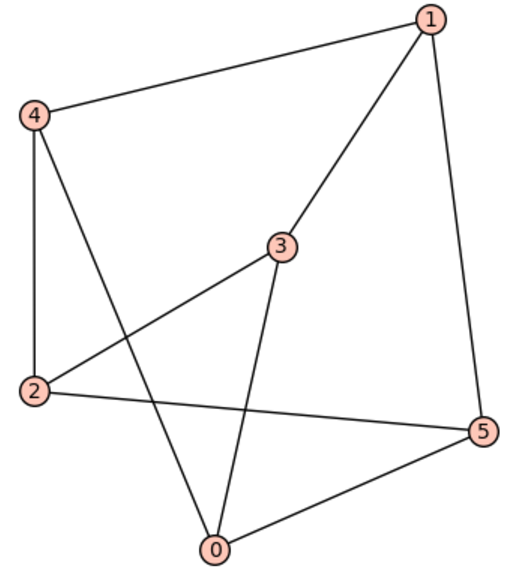
\includegraphics[width=\linewidth]{dvodelni_graf.png}
	\caption{Polni dvodelni graf na 6 vozliščih}
\end{minipage}
\hfill
\begin{minipage}{0.45\textwidth}
	\centering
	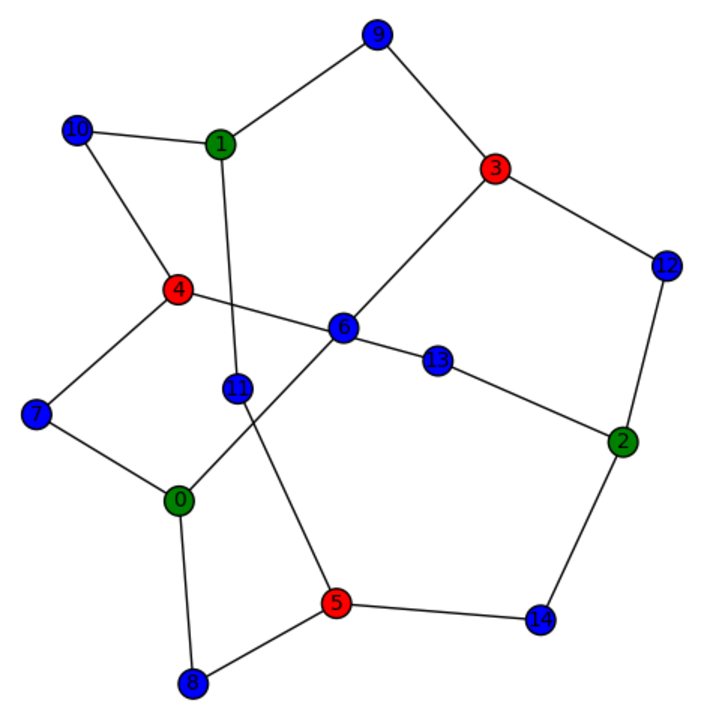
\includegraphics[width=\linewidth]{subdivizija_dvodelni_graf.png}
	\caption{Barvanje subdivizije polnega dvodelnega grafa na 6 vozliščih}
\end{minipage}
\end{figure}

\section{Stohastično iskanje}

\subsection{SAT}

Stohastičnega iskanja sva se lotila na drugačen način in sicer s t.i. \emph{"Boolean satisfiability problem"} oz. \emph{"propositional satisfiability problem"} oz.
krajše SAT iz \cite{SHAO20153588}. Deluje na principu logike, za dano logično formulo proba poiskati interpretacijo, ki zadošča formuli.  Omejitve predstavimo z logičnimi izrazi, ki jih
združimo v konjunktivno normalno obliko na katero poženemo "\textnormal{solver}". Uporabila sva MinisatGH solver. Za to metodo sva se odločila, ker je bila občutno
hitrejša kot CLP.\\
Uporabila sva sledeče omejitve:
\begin{align}
	\label{eq:f.5} & \bigvee_{i=1}^k x_{v, i} && \forall v\in V(G) \\
	\label{eq:f.6} & \neg x_{v, i} \lor \neg x_{v, j} && \forall v \in V(G), 1 \leq i < j \leq k\\
	\label{eq:f.7} & \neg x_{v, i} \lor \neg x_{u, i} && \forall u, v \in V(G), 1 \leq i \leq k
\end{align}
Pogoj $(6)$ poskrbi, da je vsako vozlišče pobarvano z vsaj eno barvo. \\
Pogoj $(7)$ poskrbi, da je vsako vozlišče pobarvano z natanko eno barvo. \\
Pogoj $(8)$ poskrbi, da sta vozlišči pobarvani z različnima barvama, če je $d_G(u, v) \leq i$.

Poleg tega nisva iskala pakirnega števila na subkubičnih grafih, temveč le na kubičnih. To pa zato, ker če je $H$ podgraf grafa $G$ je potem
$\chi_\rho(S(H)) \leq \chi_\rho(S(G))$ (to sledi iz dejstva, da je $d_H(u, v) \geq d_G(u, v)$ za vsaki vozlišči $u, v \in V(H)$) in ker je
vsak subkubičen graf podgraf nekega kubičnega. Torej če najdeva nek kubičen graf G z $\chi_\rho(S(G)) \leq 5$ bodo imeli vsi njegovi podgrafi pakirno kromatično število $\leq$ 5. Kot je bilo povedano že v prejšnjem delu, če je $G$ dvodelen pomeni, da bo $\chi_\rho(S(G)) = 3$, torej
sva ignorirala tudi dvodelne grafe.

\subsection{Lastnosti grafov pri stohastičnem iskanju}
\subsubsection{16 vozlišč}
\begin{table}[H]
	\begin{tabular}{|l|l|l|l|l|l|}
		\hline
		Število dvodelnih	& Število ravninskih  & Gostota  & Zgoščenost & Povprečna razdalja & Premer \\ \hline
		0 & 247  & 1 & 0.11 & 2.46 & 4.51 \\ \hline
	\end{tabular}
\end{table}

\subsubsection{18 vozlišč}
\begin{table}[H]
	\begin{tabular}{|l|l|l|l|l|l|}
		\hline
		Število dvodelnih	& Število ravninskih  & Gostota  & Zgoščenost & Povprečna razdalja & Premer \\ \hline
		0 & 187  & 1 & 0.095 & 2.6 & 4.8 \\ \hline
	\end{tabular}
\end{table}
\subsubsection{20 vozlišč}
\begin{table}[H]
	\begin{tabular}{|l|l|l|l|l|l|}
		\hline
		Število dvodelnih	& Število ravninskih  & Gostota  & Zgoščenost & Povprečna razdalja & Premer \\ \hline
		0 & 112  & 1 & 0.089 & 2.7 & 5.16 \\ \hline
	\end{tabular}
\end{table}
\subsubsection{22 vozlišč}
\begin{table}[H]
	\begin{tabular}{|l|l|l|l|l|l|}
		\hline
		Število dvodelnih	& Število ravninskih  & Gostota  & Zgoščenost & Povprečna razdalja & Premer \\ \hline
		0 &  53 & 1 & 0.079 & 2.86 & 5.39 \\ \hline
	\end{tabular}
\end{table}
\subsubsection{24 vozlišč}
\begin{table}[H]
	\begin{tabular}{|l|l|l|l|l|l|}
		\hline
		Število dvodelnih	& Število ravninskih  & Gostota  & Zgoščenost & Povprečna razdalja & Premer \\ \hline
		0 & 29  & 1 & 0.072 & 2.96 & 5.57 \\ \hline
	\end{tabular}
\end{table}

\subsection{Ugotovitve stohastičnega iskanja}
S povečevanjem števila vozlišč opazimo, da se količina ravninskih grafov zmanjšuje. To lahko pripišemo temu, da izbiramo med večjo količino grafov in imamo zato manjšo možnost da najdemo ravninski graf. Po pričakovanjih se premer in povprečna razdalja povečujeta ko povečujemo število vozlišč. Je pa zanimivo da se zgoščenost zmanjšuje, kar pomeni, da so povezave bolj enakomerno razporejene po grafu. Gostota pa je povsod enaka 1 saj sva generirala 3-regularne(kubične) grafe, ki pa so glede na najine predpostavke polni(imajo vse možne povezave). \\
Začetne domneve: \emph{za vsako subdivizijo subkubičnega grafa $G$ velja $\chi_\rho(S(G)) \leq 5$}, nisva ovrgla, saj nisva našla protiprimera.

\nocite{*}

\printbibliography

\end{document}